\documentclass[10pt,a4paper]{article}
\usepackage[utf8]{inputenc}
\usepackage[T1]{fontenc}
\usepackage{amsmath}
\usepackage{amsfonts}
\usepackage{amssymb}
\usepackage{graphicx}
\graphicspath{ {Imagenes/} }
\usepackage{wrapfig}
\usepackage{fancyhdr}
\usepackage{enumitem}
\usepackage{vmargin}

\setpapersize{A4}
\setmargins{2.5cm}       % margen izquierdo
{1.5cm}                        % margen superior
{16.5cm}                      % anchura del texto
{23.42cm}                    % altura del texto
{10pt}                           % altura de los encabezados
{1cm}                           % espacio entre el texto y los encabezados
{0pt}                             % altura del pie de página
{2cm}                           % espacio entre el texto y el pie de página
\begin{document}
	\title{TEMA 4: DISPOSITIVOS SEMICONDUCTORES}
	\date{}
	\author{}
	\maketitle
	
	\section{Introducción}
	\begin{itemize}
		\item Los dispositivos semiconductores son componentes electrónicos que hacen uso de las propiedades electrónicas de los materiales semiconductores.
		\item Usan la conducción eléctrica en sólidos y no en gases o la emisión termoiónica en condiciones de vacío.
		\item Se fabrican individualmente o formando partes de circuitos integrados en obleas.
		\item Como veremos, el uso de semiconductores es útil debido a que su comportamiento puede manipularse se forma sencilla añadiendo impurezas.
		\item Los semiconductores pueden ser excelentes sensores ya que su conductividad puede controlarse por distintos mecanismos (campos magnéticos, luz, calor, etc.).
		\item Los dispositivos semiconductores son las piezas básicas de las puertas lógicas, partes fundamentales de la electrónica digital.
		\item Son claves en amplificadores y osciladores en electrónica analógica.
		\item Son elementos de traducción entre circuitos digitales y analógicos.
	\end{itemize}

	\section{Materiales sólidos}
	
	\subsection{Enlaces iónicos}
	
	Los electrones están fuertemente ligados a los átomos $\implies$ aislantes.
	
	\subsection{Enlaces metálicos}
	\begin{itemize}
		\item Los electrones exteriores están desligados de los átomos, formando una nube electrónica distribuida en todo el sólido y que sirve de unión entre los núcleos atómicos.
		\item Los electrones exteriores no están ligados a ningún átomo en concreto, por lo que pueden moverse libremente bajo la acción de un campo eléctrico $\implies$ conductores.
	\end{itemize}

	\subsection{Enlaces covalentes}
	\begin{itemize}
		\item Los electrones de la capa más externa de cada átomo se comparten con otros átomos, formando un enlace entre ellos.
		\item Cada par de electrones forma un enlace entre átomos.
		\item En principio (cierto a $T = 0$K), los electrones que forman el enlace se comparten por dos átomos y no pueden desplazarse por el cristal bajo la acción de un campo eléctrico $\implies$ aislante.
		\item Al aumentar $T$, se rompen algunos enlaces, liberándose electrones que pueden moverse bajo la acción de un campo eléctrico $\implies$ conductor.
	\end{itemize}
	
	\section{Semiconductores}
	
	\subsection{Portadores: electrones y huecos}
	\begin{itemize}
		\item Al aumentar $T$, se rompen algunos enlaces liberándose electrones que pueden moverse bajo la acción de un campo eléctrico $\implies$ Formación de par electrón-hueco.
		\item Los huecos también participan en el proceso de conducción.
		\item En general, un semiconductor tiene pocos portadores libres por eso su conductividad es baja.
		\item Más portadores $\implies$ más conductividad.
	\end{itemize}
	
	\subsection{Tipos de semiconductores}
	\begin{itemize}
		\item Intrínsecos
		\item Extrínsecos (dopados)
		\begin{itemize}
			\item Tipo P (con impurezas aceptadores, materiales de la columna III).
			\item Tipo N (con impurezas donadoras, manteriales de la columna V).
		\end{itemize}
	\end{itemize}

	\section{Unión PN}
	\subsection{El diodo}
	
	\begin{itemize}
		\item Es un dispositivo de dos terminales.
		\item Símbolo:
		\begin{figure}[h]
			\centering
			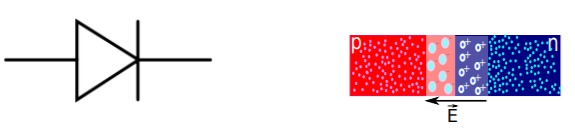
\includegraphics[scale = 0.4]{diodo}
		\end{figure}
		\item Relación voltaje/intensidad: $I_d = I_S\left(e^{\tfrac{qV_d}{k_B T}} - 1 \right)$
		
		donde $I_d$ es la intensidad que atraviesa el diodo, $I_S$ es la corriente inversa de saturación, $q$ es la carga del electrón, $V_d$ la diferencia de potencial entre los extremos del dioso, $k_B$ la constante de Boltzmann y $T$ la temperatura.
		\item Tipos de diodos: Zener, LEDs,...
	\end{itemize}

	\underline{Modelos:}
	\begin{itemize}
		\item \textbf{Modelo 1.} El diodo se comporta como una fuente de tensión de valor $V_\gamma$.
		\item \textbf{Modelo 2.} El diodo se comporta en conducción como una fuente de tensión $V_\gamma$, en serie con una resistencia $r_d$.
	\end{itemize}
	
	\begin{minipage}{0.45\linewidth}
		\vspace*{0pt}
		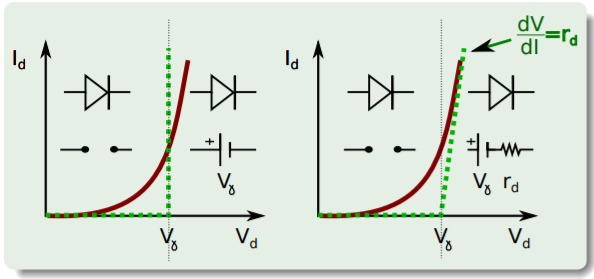
\includegraphics[scale = 0.35]{modelos_1}
	\end{minipage}%
	\begin{minipage}{0.55\linewidth}
		\vspace*{0pt}
		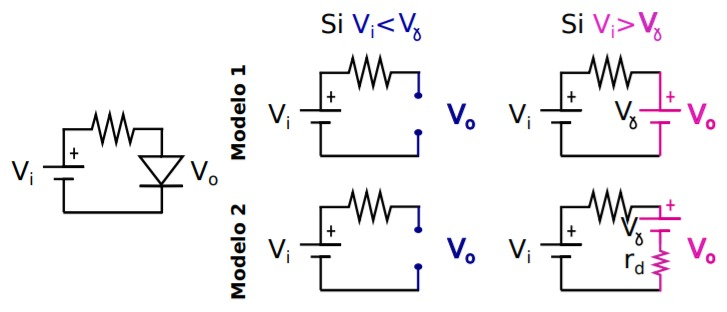
\includegraphics[scale = 0.35]{modelos_2}
	\end{minipage}
	
	\newpage
	\underline{Característica de transferencia:} \newline
	
	Es la representación de la salida de un circuito en función de la entrada.
	
	\begin{figure}[h]
		\centering
		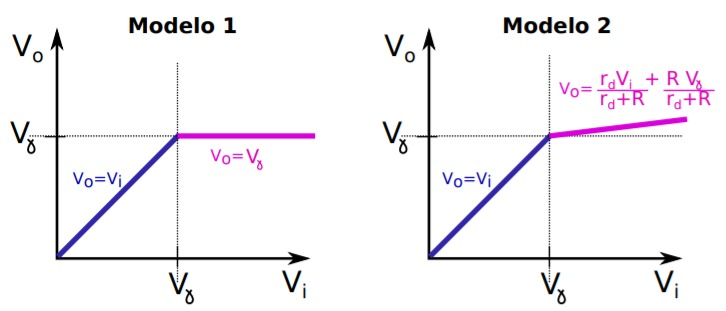
\includegraphics[scale=0.5]{caracteristica_trans}
	\end{figure}

	\section{El transistor MOSFET}
	
	\begin{itemize}
		\item Dispositivo electrónico de tres terminales llamados puerta ($G$, gate), drenador ($D$, drain) y fuente ($S$, source).
		\item La corriente fluye entre la fuente y el drenador y se controla con la tensión aplicada en la puerta.
	\end{itemize}
	
	\subsection{Modo de funcionamiento: CORTE}
	
	\begin{itemize}
		\item \textbf{Objetivo: }que los electrones circulen desde $S$ a $D \implies V_D > V_S$.
		\item En \textbf{corte}: $V_G - V_S = V_{GS} < V_T$.
		\item Si $V_G - V_S = V_{GS} < V_T \implies$ no hay capa de inversión en $S$ ni en $D \implies$ no hay canal entre ellos.
	\end{itemize}
	\vspace{0cm}
	\begin{itemize}
		\item Ocurre si $V_{GS} \leq V_T$
		\item El transistor está OFF porque no hay canal.
		\item No hay conducción entre drenador y fuente ($I_D = 0$).
		\item $I_G = 0$.
		\item Corriente de fuga.
	\end{itemize}
	
	\subsection{Modo de funcionamiento: LINEAL}
	
	\begin{itemize}
		\item \textbf{Objetivo: }que los electrones circulen desde $S$ a $D \implies V_D > V_S$.
		\item En \textbf{lineal: }$V_{GS} > V_T$ y $V_{DS} < V_{GS} - V_T$.
		\item $V_G - V_S = V_{GS} > V_T \implies$ hay capa de inversión en $S$.
		\item Si $V_D - V_S < V_G - V_S - V_T \implies V_T < V_G - V_D = V_{GD} \implies$ hay capa de inversión en D.
		\item Hay canal entre $S$ y $D$, y los electrones van desde S a D.
	\end{itemize}
	
	\vspace*{1cm}
	
	\begin{itemize}
		\item Ocurre si $V_{GS} > V_T$ y $V_{DS} < V_{GS} - V_T$
		\item El transistor está ON.
		\item $I_G = 0$.
		\item Hay conducción entre drenador y fuente: $$I_D = \dfrac{k}{2}[2(V_{GS} - V_T)V_{DS} - V_{DS}^2]$$.
	\end{itemize}

	\subsection{Modo de funcionamiento: SATURACIÓN}
	
	
	\begin{itemize}
		\item \textbf{Objetivo: }que los electrones circulen desde S a D $\implies V_D > V_S$.
		\item En \textbf{saturación: }$V_{GS} > V_T$ y $V_{DS} > V_{GS} - V_T$.
		\item Si $V_G - V_S = V_{GS} > V_T \implies$ hay capa de inversión en S.
		\item Si $V_D - V_S > V_G - V_S - V_T \implies V_T > V_G - V_D = V_{GD} \implies$ no hay capa de inversión en D.
		\item La capa de inversión que hay en S se hace cada vez más estrecha al acercarnos a D. A pesar de que el canal no ocupa toda la zona entre S y D, los electrones van de S a D.
	\end{itemize}
	\vspace*{0pt}
	\begin{itemize}
		\item Ocurre si $V_{GS} > V_T$ y $V_{DS} > V_{GS} - V_T$.
		\item El transistor está ON.
		\item $I_G = 0$.
		\item Hay conducción entre drenador y fuente: $$I_D = \dfrac{k}{2}(V_{GS} - V_T)^2$$
	\end{itemize}

	\subsection{Funcionamiento de pMOSFET}
	
	Tiene los mismos 3 modos de funcionamiento que el nMOSFET, y las ecuaciones son las mismas pero con las variables en valor absoluto.
\end{document}